\documentclass[aspectratio=169,10pt]{beamer}

% Theme
\usetheme{Madrid}
\usecolortheme{default}
\setbeamertemplate{navigation symbols}{}
\setbeamertemplate{footline}[frame number]

% Packages
\usepackage{amsmath,amssymb}
\usepackage{booktabs}
\usepackage{tikz}
\usetikzlibrary{arrows.meta,positioning,shapes.geometric,calc}
\usepackage{algorithm2e}
\usepackage{xcolor}
\usepackage{graphicx}
\graphicspath{{images/}}

% Colors
\definecolor{boundary}{RGB}{220,53,69}
\definecolor{episode1}{RGB}{40,167,69}
\definecolor{episode2}{RGB}{0,123,255}
\definecolor{episode3}{RGB}{255,193,7}

% Title
\title{Unsupervised Episode Detection for Scene Graph Understanding}
\author{}
\date{}

\begin{document}

%==============================================================================
\begin{frame}
\titlepage
\end{frame}

%==============================================================================
\begin{frame}{Why Scene Graphs?}

\textbf{Scene graphs}: Structured representation encoding entities, attributes, and relationships

\vspace{0.3cm}
\textbf{Key Benefits}:
\begin{itemize}
\item Enable \textbf{spatial and temporal reasoning} in multimodal settings
\item Provide \textbf{grounding for LLMs} in embodied AI and robotics
\item Bridge gap between visual perception and symbolic reasoning
\item Support complex queries about actions, objects, and relationships
\end{itemize}

\vspace{0.3cm}
\textbf{The Challenge} (Yang et al., 2025):
\begin{itemize}
\item LLMs can \textit{understand} scene graphs reasonably well
\item But \textbf{struggle to generate} them from complex narratives
\item Difficulty decomposing narratives into discrete scenes
\end{itemize}

\vspace{0.3cm}
\small
\textit{``Scene graphs provide essential grounding for LLMs in spatial and temporal understanding within multimodal environments.''}

\end{frame}

%==============================================================================
\begin{frame}{Video Scene Graph: Definition}

\begin{center}
\includegraphics[width=0.50\textwidth]{video_scene_graph_definition.png}
\end{center}

\small
\textbf{Structure}: Each action is a graph: \textbf{Agent} $\xrightarrow{\text{verb}}$ \textbf{Action} $\xrightarrow{\text{dobj}}$ \textbf{Object}, with \texttt{with}, \texttt{of}, \texttt{into} relations

\hfill\scriptsize Figure from Yang et al. (ACL 2025)

\end{frame}

%==============================================================================
\begin{frame}{SGQA: Scene Graph Question Answering}

\begin{center}
\includegraphics[width=0.75\textwidth]{SGQA_demo.png}
\end{center}

\small
\textbf{Task}: Answer temporal reasoning questions over action graph sequences\\
Requires understanding \textbf{action order} (``before'', ``after'', ``between'') and \textbf{object relationships}

\hfill\scriptsize Figure from Yang et al. (ACL 2025)

\end{frame}

%==============================================================================
\begin{frame}{Abstract}
\small
Scene graphs represent activities as flat sequences of action triplets, lacking the hierarchical structure needed for temporal reasoning. We present an unsupervised approach that detects episode boundaries through \textbf{co-occurrence pattern shifts}.

\vspace{0.3cm}
Our method:
\begin{enumerate}
\item Computes term \textbf{salience} against a background corpus
\item Builds action similarity matrices using \textbf{Jaccard coefficients}
\item Identifies boundaries where consecutive similarity drops below $\mu - \sigma$
\item Refines boundaries into structured episodes via \textbf{LLM labeling}
\end{enumerate}

\vspace{0.3cm}
On SGQA (500 questions), this hybrid statistical-semantic approach improves exact match accuracy from \textbf{88.6\%} to \textbf{90.6\%}. On Hard-10 (difficult cases), accuracy improves from \textbf{20\%} to \textbf{50\%}.
\end{frame}

%==============================================================================
\begin{frame}{Problem: Flat Scene Graphs Lack Structure}

\textbf{Scene graphs} represent actions as sequences of triplets:
\begin{center}
\small
\texttt{[person, verb, pick-up], [pick-up, dobj, mop], [mop, from, floor], ...}
\end{center}

\vspace{0.3cm}
\textbf{Challenge}: Temporal reasoning requires understanding \textbf{episode boundaries}

\vspace{0.3cm}
\begin{columns}
\begin{column}{0.48\textwidth}
\textbf{Without hierarchy:}
\begin{itemize}
\item Flat sequence of 11 actions
\item No phase structure
\item Model must infer relationships
\end{itemize}
\end{column}
\begin{column}{0.48\textwidth}
\textbf{With hierarchy:}
\begin{itemize}
\item Episode 1: Prepare \& sweep
\item Episode 2: Store supplies
\item Episode 3: Retrieve from cabinet
\end{itemize}
\end{column}
\end{columns}

\vspace{0.3cm}
\textbf{Key Question}: How to detect meaningful phases \textit{without supervision}?

\end{frame}

%==============================================================================
\begin{frame}{Our Approach: EpiMine for Scene Graphs}

\textbf{Key Insight}: Episodes detected via \textbf{co-occurrence pattern shifts}

\vspace{0.3cm}
\begin{center}
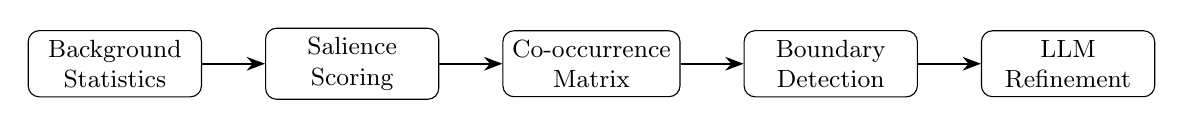
\begin{tikzpicture}[
    node distance=0.8cm,
    box/.style={rectangle, draw, rounded corners, minimum width=2.2cm, minimum height=0.7cm, align=center, font=\small},
    arrow/.style={-{Stealth}, thick}
]
\node[box] (bg) {Background\\Statistics};
\node[box, right=of bg] (sal) {Salience\\Scoring};
\node[box, right=of sal] (cooc) {Co-occurrence\\Matrix};
\node[box, right=of cooc] (bound) {Boundary\\Detection};
\node[box, right=of bound] (llm) {LLM\\Refinement};

\draw[arrow] (bg) -- (sal);
\draw[arrow] (sal) -- (cooc);
\draw[arrow] (cooc) -- (bound);
\draw[arrow] (bound) -- (llm);
\end{tikzpicture}
\end{center}

\vspace{0.3cm}
\textbf{Hybrid approach}:
\begin{itemize}
\item \textbf{Statistical}: Unsupervised boundary detection (reproducible)
\item \textbf{Semantic}: LLM generates episode names/descriptions
\end{itemize}

\end{frame}

%==============================================================================
\begin{frame}{Step 1: Salience -- Identifying Discriminative Terms}

\textbf{Goal}: Find terms that characterize the current activity

\vspace{0.2cm}
\textbf{Formula}:
\[
\text{salience}(t) = \underbrace{(1 + \log(f_{\text{fg}})^2)}_{\text{foreground boost}} \times \underbrace{\log\left(\frac{N_{\text{bg}}}{f_{\text{bg}}}\right)}_{\text{IDF component}}
\]

\vspace{0.1cm}
\begin{itemize}
\item $f_{\text{fg}}$: term frequency in current sample (foreground)
\item $f_{\text{bg}}$: term frequency across all samples (background)
\end{itemize}

\vspace{0.2cm}
\begin{columns}
\begin{column}{0.55\textwidth}
\textbf{Example} (Car Cleaning):
\begin{center}
\small
\begin{tabular}{lcc}
\toprule
\textbf{Term} & \textbf{Salience} & \textbf{Interpretation} \\
\midrule
mop-stick & 18.86 & Highly discriminative \\
wall & 9.98 & Discriminative \\
person & $\approx 0$ & Common (filtered) \\
\bottomrule
\end{tabular}
\end{center}
\end{column}
\begin{column}{0.42\textwidth}
\colorbox{blue!10}{
\parbox{0.95\textwidth}{
\small
\textbf{Tunable: \texttt{min\_freq}}\\[0.1cm]
Filter terms with $f_{\text{fg}} < $ \texttt{min\_freq}\\[0.1cm]
\textit{Higher} $\rightarrow$ fewer episodes\\
\textbf{Optimal}: \texttt{min\_freq=2}
}}
\end{column}
\end{columns}

\end{frame}

%==============================================================================
\begin{frame}{Step 2: Co-occurrence Matrix}

\textbf{Goal}: Measure similarity between consecutive actions using top-$k$ salient terms

\vspace{0.2cm}
\textbf{Jaccard Similarity} (using only top-$k$ key terms):
\[
\text{cooccur}(A_i, A_j) = \frac{|\text{terms}_k(A_i) \cap \text{terms}_k(A_j)|}{|\text{terms}_k(A_i) \cup \text{terms}_k(A_j)|}
\]

\vspace{0.2cm}
\begin{columns}
\begin{column}{0.55\textwidth}
\textbf{Intuition}:
\begin{itemize}
\item \textbf{High co-occurrence} $\rightarrow$ same episode
\item \textbf{Low co-occurrence} $\rightarrow$ boundary
\end{itemize}

\vspace{0.2cm}
\begin{center}
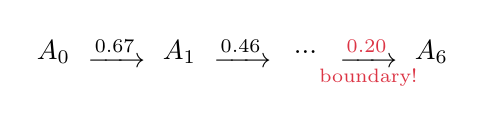
\begin{tikzpicture}[scale=0.8]
\node at (0,0) {$A_0$};
\node at (1.0,0) {$\xrightarrow{0.67}$};
\node at (2.0,0) {$A_1$};
\node at (3.0,0) {$\xrightarrow{0.46}$};
\node at (4.0,0) {...};
\node at (5.0,0) {$\xrightarrow{\textcolor{boundary}{0.20}}$};
\node at (6.0,0) {$A_6$};
\node[font=\scriptsize,text=boundary] at (5.0,-0.4) {boundary!};
\end{tikzpicture}
\end{center}
\end{column}
\begin{column}{0.42\textwidth}
\colorbox{blue!10}{
\parbox{0.95\textwidth}{
\small
\textbf{Tunable: \texttt{top\_k}}\\[0.1cm]
Limit to top-$k$ salient terms\\[0.1cm]
\texttt{topk=all}: noisy (18.3\% avg)\\
\texttt{topk=5}: too sparse (20.8\%)\\
\textbf{Optimal}: \texttt{topk=10} (24.2\%)
}}
\end{column}
\end{columns}

\end{frame}

%==============================================================================
\begin{frame}{Step 3: Boundary Detection}

\begin{columns}
\begin{column}{0.55\textwidth}
\textbf{Algorithm}:
\begin{enumerate}
\item Compute consecutive scores: $s_i = \text{cooccur}(A_i, A_{i+1})$
\item Calculate threshold: $\tau = \mu - t \cdot \sigma$
\item If $s_i < \tau$: start new episode
\end{enumerate}

\vspace{0.2cm}
\textbf{Example} (11 actions):
\begin{center}
\scriptsize
\begin{tabular}{cccccc}
\toprule
$A_0{\to}A_1$ & ... & $A_5{\to}A_6$ & ... & $A_9{\to}A_{10}$ \\
\midrule
0.67 & ... & \textcolor{boundary}{\textbf{0.20}} & ... & \textcolor{boundary}{\textbf{0.31}} \\
\bottomrule
\end{tabular}
\end{center}

$\tau = 0.437 - 1.0 \times 0.129 = 0.308$
\end{column}
\begin{column}{0.42\textwidth}
\colorbox{blue!10}{
\parbox{0.95\textwidth}{
\small
\textbf{Tunable: \texttt{threshold\_std}}\\[0.1cm]
Formula: $\tau = \mu - t \cdot \sigma$\\[0.1cm]
Lower $t$ $\rightarrow$ more boundaries\\
Higher $t$ $\rightarrow$ fewer episodes\\[0.1cm]
\begin{tabular}{lcc}
\scriptsize $t$ & \scriptsize Avg & \scriptsize Max \\
\scriptsize 1.0 & \scriptsize 15.8\% & \scriptsize 30\% \\
\scriptsize \textbf{1.5} & \scriptsize \textbf{24.2\%} & \scriptsize \textbf{50\%} \\
\scriptsize 2.0 & \scriptsize 23.3\% & \scriptsize 30\% \\
\end{tabular}
}}
\end{column}
\end{columns}

\vspace{0.2cm}
\textbf{Detected Episodes}:
\begin{itemize}
\item \textcolor{episode1}{Episode 0}: Actions [0-5] -- pick-up, sweep, close, place, open, put
\item \textcolor{episode2}{Episode 1}: Actions [6-9] -- move, open, pick-up, move
\item \textcolor{episode3}{Episode 2}: Action [10] -- pick
\end{itemize}

\end{frame}

%==============================================================================
\begin{frame}[fragile]{Step 4: LLM Refinement}

\textbf{LLM refines boundaries into structured episodes}:

\vspace{0.1cm}
\begin{columns}
\begin{column}{0.55\textwidth}
\small
\begin{verbatim}
{
  "episode_id": 0,
  "name": "Prepare and Sweep",
  "description": "Pick up mop,
    sweep floor, manage door",
  "core_structure": {
    "agent": "person",
    "actions": ["pick-up","sweep"],
    "objects": ["mop-stick","floor"]
  },
  "time": {
    "action_indices": [0,1,2,3,4,5],
    "duration": 6
  }
}
\end{verbatim}
\end{column}
\begin{column}{0.42\textwidth}
\colorbox{blue!10}{
\parbox{0.95\textwidth}{
\small
\textbf{Tunable: \texttt{use\_llm}, \texttt{gen\_model}}\\[0.1cm]
\texttt{use\_llm=0}: structural only\\
\texttt{use\_llm=1}: semantic naming\\[0.1cm]
\texttt{gen\_model}: gpt5-mini vs gpt5\\[0.1cm]
\begin{tabular}{lcc}
\scriptsize Setting & \scriptsize Avg & \scriptsize Max \\
\scriptsize noLLM & \scriptsize 18.9\% & \scriptsize 30\% \\
\scriptsize \textbf{LLM} & \scriptsize \textbf{23.3\%} & \scriptsize \textbf{50\%} \\
\end{tabular}\\[0.1cm]
\textit{+4.4\% avg improvement}
}}
\end{column}
\end{columns}

\vspace{0.2cm}
\textbf{Output}: Episode name, description, core structure, temporal info, discriminative terms

\end{frame}

%==============================================================================
\begin{frame}{Hard-10 Benchmark: Targeting Difficult Questions}

\textbf{Motivation}: General SGQA accuracy (88.6\%) may hide weaknesses

\vspace{0.3cm}
\textbf{Construction}:
\begin{enumerate}
\item Run GPT-5 on full SGQA (500 questions)
\item Identify \textbf{88 questions} where GPT-5 failed
\item Select \textbf{first 10} for rapid hyperparameter iteration
\end{enumerate}

\vspace{0.3cm}
\textbf{Hard Question Categories}:
\begin{center}
\small
\begin{tabular}{lcc}
\toprule
\textbf{Category} & \textbf{Count} & \textbf{Example} \\
\midrule
temporal\_ordering & 57 & ``What was done \textit{before} X?'' \\
multi\_step & 17 & ``After completing sequence A...'' \\
both\_hands & 9 & ``Which object required both hands?'' \\
\bottomrule
\end{tabular}
\end{center}

\vspace{0.3cm}
\textbf{Baseline}: GPT-5 on Hard-10 = \textbf{20\%} (2/10 correct)

\end{frame}

%==============================================================================
\begin{frame}{Pipeline with Tunable Parameters}

\begin{center}
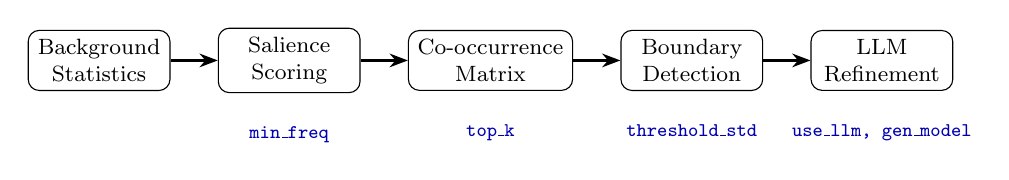
\begin{tikzpicture}[
    node distance=0.6cm,
    box/.style={rectangle, draw, rounded corners, minimum width=1.8cm, minimum height=0.6cm, align=center, font=\footnotesize},
    param/.style={font=\scriptsize\ttfamily, text=blue!70!black},
    arrow/.style={-{Stealth}, thick}
]
\node[box] (bg) {Background\\Statistics};
\node[box, right=of bg] (sal) {Salience\\Scoring};
\node[box, right=of sal] (cooc) {Co-occurrence\\Matrix};
\node[box, right=of cooc] (bound) {Boundary\\Detection};
\node[box, right=of bound] (llm) {LLM\\Refinement};

\draw[arrow] (bg) -- (sal);
\draw[arrow] (sal) -- (cooc);
\draw[arrow] (cooc) -- (bound);
\draw[arrow] (bound) -- (llm);

% Parameter annotations
\node[param, below=0.3cm of sal] (p1) {min\_freq};
\node[param, below=0.3cm of cooc] (p2) {top\_k};
\node[param, below=0.3cm of bound] (p3) {threshold\_std};
\node[param, below=0.3cm of llm] (p4) {use\_llm, gen\_model};
\end{tikzpicture}
\end{center}

\vspace{0.2cm}
\begin{center}
\small
\begin{tabular}{llll}
\toprule
\textbf{Parameter} & \textbf{Step} & \textbf{Effect} & \textbf{Range} \\
\midrule
\texttt{min\_freq} & Salience & Filter rare terms & 1, 2 \\
\texttt{top\_k} & Co-occurrence & Limit key terms & 5, 10, all \\
\texttt{threshold\_std} & Boundary & Sensitivity ($\mu - t \cdot \sigma$) & 1.0, 1.5, 2.0 \\
\texttt{use\_llm} & LLM & Enable episode naming & 0, 1 \\
\texttt{gen\_model} & LLM & Model for naming & gpt5-mini, gpt5 \\
\bottomrule
\end{tabular}
\end{center}

\end{frame}

%==============================================================================
\begin{frame}{Grid Search Design}

\textbf{Goal}: Find optimal parameter combination on Hard-10

\vspace{0.3cm}
\begin{center}
\begin{tabular}{ll}
\toprule
\textbf{Parameter} & \textbf{Values} \\
\midrule
\texttt{threshold\_std} & 1.0, 1.5, 2.0 \\
\texttt{min\_freq} & 1, 2 \\
\texttt{top\_k} & 5, 10, all \\
\texttt{use\_llm} & 0 (structural), 1 (LLM naming) \\
\bottomrule
\end{tabular}
\end{center}

\vspace{0.3cm}
\textbf{Total experiments}: $3 \times 2 \times 3 \times 2 = \textbf{36}$

\vspace{0.3cm}
\textbf{Evaluation metric}: Exact Match accuracy on 10 hard questions

\vspace{0.3cm}
\textbf{Question}: Which parameter combination maximizes accuracy?

\end{frame}

%==============================================================================
\begin{frame}{Grid Search Results: Best Configurations}

\begin{center}
\begin{tabular}{cccccc}
\toprule
\textbf{Rank} & \textbf{Accuracy} & \textbf{threshold} & \textbf{min\_freq} & \textbf{top\_k} & \textbf{LLM} \\
\midrule
1 & \textcolor{episode1}{\textbf{50\%}} & 1.5 & 2 & 10 & Yes \\
2 & \textcolor{episode2}{\textbf{40\%}} & 1.5 & 2 & 5 & Yes \\
3-11 & 30\% & various & various & 5,10 & mixed \\
\midrule
Baseline & 20\% & -- & -- & -- & -- \\
\bottomrule
\end{tabular}
\end{center}

\vspace{0.3cm}
\textbf{Key findings}:
\begin{itemize}
\item Best config achieves \textbf{+150\% relative improvement} (20\% $\rightarrow$ 50\%)
\item Both top configs share: \texttt{threshold=1.5}, \texttt{min\_freq=2}, \texttt{llm=1}
\item Parameter \textbf{interaction effects} matter (no single param dominates)
\end{itemize}

\end{frame}

%==============================================================================
\begin{frame}{Parameter Impact Analysis}

\begin{columns}
\begin{column}{0.48\textwidth}
\textbf{1. threshold\_std} (Boundary Sensitivity)
\small
\begin{tabular}{lccc}
\toprule
Value & Avg & Max & Episodes \\
\midrule
t=1.0 & 15.8\% & 30\% & More \\
\textbf{t=1.5} & \textbf{24.2\%} & \textbf{50\%} & \textbf{Moderate} \\
t=2.0 & 23.3\% & 30\% & Fewer \\
\bottomrule
\end{tabular}

\vspace{0.1cm}
\scriptsize\textit{Formula: $\tau = \mu - t \cdot \sigma$. Lower $t$ $\rightarrow$ more boundaries.}

\vspace{0.15cm}
\small
\textbf{2. top\_k} (Key Term Limit)
\small
\begin{tabular}{lcc}
\toprule
Value & Avg & Max \\
\midrule
topk=5 & 20.8\% & 40\% \\
\textbf{topk=10} & \textbf{24.2\%} & \textbf{50\%} \\
topk=all & 18.3\% & 30\% \\
\bottomrule
\end{tabular}
\end{column}

\begin{column}{0.48\textwidth}
\textbf{3. min\_freq} (Term Filtering)
\small
\begin{tabular}{lcc}
\toprule
Value & Avg & Max \\
\midrule
mf=1 & 21.7\% & 30\% \\
\textbf{mf=2} & 20.6\% & \textbf{50\%} \\
\bottomrule
\end{tabular}

\vspace{0.3cm}
\textbf{4. use\_llm} (Episode Naming)
\small
\begin{tabular}{lcc}
\toprule
Value & Avg & Max \\
\midrule
noLLM & 18.9\% & 30\% \\
\textbf{LLM} & \textbf{23.3\%} & \textbf{50\%} \\
\bottomrule
\end{tabular}

\vspace{0.2cm}
\textit{+4.4\% avg improvement}
\end{column}
\end{columns}

\end{frame}

%==============================================================================
\begin{frame}{LLM Impact: Threshold-Dependent}

\textbf{LLM helps most at optimal threshold (t=1.5)}

\vspace{0.2cm}
\begin{center}
\small
\begin{tabular}{lcccc}
\toprule
\textbf{Config} & \textbf{noLLM} & \textbf{LLM} & \textbf{$\Delta$} \\
\midrule
t=1.5, mf=2, topk=10 & 20\% & \textbf{50\%} & \textcolor{episode1}{+30\%} \\
t=1.5, mf=2, topk=5 & 10\% & \textbf{40\%} & \textcolor{episode1}{+30\%} \\
t=1.5, mf=1, topk=10 & 10\% & 30\% & \textcolor{episode1}{+20\%} \\
\midrule
t=1.0, mf=1, topk=10 & 30\% & 10\% & \textcolor{boundary}{-20\%} \\
t=2.0, mf=2, topk=10 & 30\% & 20\% & \textcolor{boundary}{-10\%} \\
\bottomrule
\end{tabular}
\end{center}

\vspace{0.3cm}
\textbf{Analysis} (18 paired comparisons):
\begin{itemize}
\item LLM \textbf{improved} 7 configs (avg +18.6\% when it helps)
\item LLM \textbf{degraded} 4 configs (avg -12.5\% when it hurts)
\item LLM \textbf{no change} 7 configs
\end{itemize}

\vspace{0.2cm}
\textbf{Insight}: LLM episode naming amplifies good boundaries, but can hurt poor ones

\end{frame}

%==============================================================================
\begin{frame}{Results Summary}

\begin{columns}
\begin{column}{0.48\textwidth}
\textbf{Full SGQA} (500 questions)
\begin{center}
\small
\begin{tabular}{lcc}
\toprule
\textbf{Method} & \textbf{EM} & \textbf{Diff} \\
\midrule
Baseline & 88.6\% & -- \\
EpiMine (gen5-mini) & 89.6\% & +1.0\% \\
EpiMine (gen5) & \textbf{90.6\%} & \textcolor{episode1}{+2.0\%} \\
\bottomrule
\end{tabular}
\end{center}

\vspace{0.2cm}
\small
\begin{itemize}
\item Config: t=1.5, mf=2, topk=10
\item gen5 slightly better (+1\%)
\end{itemize}
\end{column}

\begin{column}{0.48\textwidth}
\textbf{Hard-10 Benchmark} (10 questions)
\begin{center}
\small
\begin{tabular}{lcc}
\toprule
\textbf{Method} & \textbf{EM} & \textbf{Diff} \\
\midrule
Baseline & 20\% & -- \\
EpiMine (gen5-mini) & \textbf{50\%} & \textcolor{episode1}{+30\%} \\
EpiMine (gen5) & 40\% & +20\% \\
\bottomrule
\end{tabular}
\end{center}

\vspace{0.2cm}
\small
\begin{itemize}
\item +150\% relative gain (best)
\item gen5-mini better than gen5!
\end{itemize}
\end{column}
\end{columns}

\vspace{0.4cm}
\textbf{Key insight}: EpiMine shows larger gains on \textit{harder} questions; gen\_model choice matters

\end{frame}

%==============================================================================
\begin{frame}{Optimal Hyperparameters (54 Experiments)}

\begin{center}
\begin{tabular}{llll}
\toprule
\textbf{Parameter} & \textbf{Range} & \textbf{Optimal} & \textbf{Why} \\
\midrule
\texttt{threshold\_std} & 1.0, 1.5, 2.0 & \textbf{1.5} & Moderate boundary sensitivity \\
\texttt{min\_freq} & 1, 2 & \textbf{2} & Filter noise, keep signal \\
\texttt{top\_k} & 5, 10, all & \textbf{10} & Focus on key terms \\
\texttt{use\_llm} & 0, 1 & \textbf{1} & +4.4\% avg improvement \\
\texttt{gen\_model} & gpt5-mini, gpt5 & \textbf{task-dep.} & See analysis below \\
\bottomrule
\end{tabular}
\end{center}

\vspace{0.3cm}
\textbf{Grid search insights}:
\begin{itemize}
\item \texttt{threshold\_std=1.5}: Not too sensitive (1.0), not too coarse (2.0)
\item \texttt{top\_k=all} hurts performance (noise from irrelevant terms)
\item LLM impact is \textbf{threshold-dependent}: helps at t=1.5, can hurt elsewhere
\item \texttt{gen\_model}: gen5-mini better on Hard-10, gen5 better on Full SGQA
\end{itemize}

\vspace{0.3cm}
\textbf{Best config}: t=1.5, mf=2, topk=10, llm=1 $\rightarrow$ \textbf{50\%} on Hard-10 (gen5-mini), \textbf{90.6\%} on Full SGQA (gen5)

\end{frame}

%==============================================================================
\begin{frame}{Gen\_model Impact: Task-Dependent}

\textbf{Does a larger LLM for episode naming help?}

\vspace{0.3cm}
\begin{columns}
\begin{column}{0.48\textwidth}
\textbf{Hard-10 Benchmark} (18 paired comparisons)
\begin{center}
\small
\begin{tabular}{lcc}
\toprule
\textbf{Gen Model} & \textbf{Avg} & \textbf{Max} \\
\midrule
\textbf{gen5-mini} & \textbf{23.3\%} & \textbf{50\%} \\
gen5 & 20.6\% & 40\% \\
\bottomrule
\end{tabular}
\end{center}

\vspace{0.1cm}
\small
Improvements: 4, Same: 5, Regressions: 9

\vspace{0.2cm}
\textit{Smaller model wins on hard cases!}
\end{column}

\begin{column}{0.48\textwidth}
\textbf{Full SGQA} (500 questions)
\begin{center}
\small
\begin{tabular}{lcc}
\toprule
\textbf{Gen Model} & \textbf{t=1.5, topk=10} & \textbf{topk=5} \\
\midrule
gen5-mini & 89.6\% & 89.4\% \\
\textbf{gen5} & \textbf{90.6\%} & 89.0\% \\
\bottomrule
\end{tabular}
\end{center}

\vspace{0.2cm}
\textit{Larger model helps on easier cases}
\end{column}
\end{columns}

\vspace{0.4cm}
\textbf{Hypothesis}: gen5-mini's concise naming better matches Hard-10's temporal reasoning needs; gen5's richer descriptions help general QA

\end{frame}

%==============================================================================
\begin{frame}{Future Directions}

\begin{enumerate}
\item \textbf{Refined hierarchical structure}
\begin{itemize}
\item Improve episode detection algorithms
\item Define better hierarchical representation for video scene graphs
\item Nested episodes, scene-level abstraction
\end{itemize}

\vspace{0.3cm}
\item \textbf{Multimodal integration}
\begin{itemize}
\item Incorporate visual features from video frames
\item Combine symbolic scene graphs with perceptual signals
\item Ground episode boundaries in visual cues
\end{itemize}

\vspace{0.3cm}
\item \textbf{Graph-based reasoning for long-form video}
\begin{itemize}
\item Leverage graph structure for complex temporal reasoning
\item Scale to hour-long videos with hierarchical decomposition
\item Enable multi-hop reasoning across episodes
\end{itemize}
\end{enumerate}

\end{frame}

\end{document}
